\documentclass[12pt,a4paper]{article}
\usepackage[utf8]{inputenc}
\usepackage[german]{babel}
\usepackage[T1]{fontenc}
\usepackage{amsmath}
\usepackage{amsfonts}
\usepackage{amssymb}
\usepackage{graphicx}
\usepackage{lmodern}
\usepackage[left=2cm,right=2cm,top=3cm,bottom=2cm]{geometry}
\usepackage{scrlayer-scrpage}
\usepackage[shortlabels]{enumitem}
\usepackage{venndiagram}

\pagestyle{headings}
\ihead{Diskrete Mathematik, HS 2020\\Prof. Christian Cachin}
\ohead{Pascale Welsch\\13-204-821}
\begin{document}
\section*{Übung 4}
\subsection*{4.1 Mengen}
\begin{enumerate}[a)]
\item Die Menge $A\cup C$ enthält alle Elemente, die in $A$ oder in $C$ enthalten sind: $$\{x|x\in A \lor x \in C\}.$$
Die Menge $B \cup C$ enthält alle Elemente, die in $B$ oder $C$ enthalten sind: $$\{x | x \in B \lor x \in C\}.$$
Wenn gilt, dass $A\cup C = B\cup C$, so müssen alle Elemente der beiden Vereinigungsmengen, die \textbf{nicht} in $C$ enthalten sind, in $A$ \textbf{und} auch in $B$ enthalten sein und keine der beiden Mengen $A$ oder $B$ darf noch zusätzliche Elemente enthalten. Damit gilt $$(A \cup C = B \cup C) \Leftrightarrow (A = B) \equiv \text{ TRUE}.$$
\begin{center}
\begin{venndiagram2sets}[labelB=$C$]
\fillA
\fillB
\end{venndiagram2sets}
\begin{venndiagram2sets}[labelA=$B$, labelB = $C$]
\fillA
\fillB
\end{venndiagram2sets}
\end{center}
\item $(A \subseteq B) \Leftrightarrow (\overline{B} \subseteq \overline{A}) \equiv \text{TRUE}$\\
\begin{center}
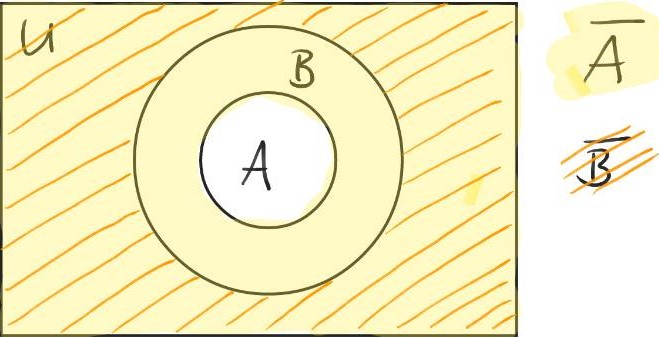
\includegraphics[width=0.4\textwidth]{venn.jpg}
\end{center}
Dies gilt auch, wenn $A$ keine \textbf{echte} Teilmenge von $B$ ist, vorausgesetzt das Universum ist für beide Mengen identisch.
\item Als Grundmenge kämen hier nur die Mengen $\{a\}$ und $\{\varnothing , a\}$ in Frage, da die Grundmenge alle (Einzel-)elemente enthalten muss, die auch in der Potenzmengen enthalten sind.
$$P(\{a\}) = \{\varnothing , \{a\}\} \text{ und } P(\{\varnothing , \{a\},\{\varnothing\}, \{\varnothing , a\}\})$$
Also ergibt keine der beiden Mengen die Potenzmenge aus der Aufgabenstellung. Zudem muss die Kardinalität einer Potenzmenge immer eine Zweierpotenz sein. Auch dass ist hier nicht gegeben. Deshalb ist diese Aussage FALSE.
\item Wie bereits bei c) gezeigt, ist dies die Potenzmenge von $\{\varnothing , a\}$. Diese Aussage ist also TRUE.
\end{enumerate}
\subsection*{4.2 Mengendifferenzen}
Die Identität der beiden Mengen $(A-B)-C$ und $(A-C)-(B-C)$ wird direkt gezeigt, indem dafür die Mengenidentitäten aus dem Lehrbuch (Rosen, 7th edition, S. 130) verwendet werden. Zusätzlich wird die folgende Identität verwendet:
\begin{align}
A-B = \{x | x \in A \land x \not\in B\} = A\cap \overline{B} 
\end{align}
\begin{align*}
(A-C)-(B-C) & \stackrel{(1)}{=} (A\cap \overline{C}) - (B \cap \overline{C})~|~(1)\\
&= (A\cap \overline{C}) \cap\overline{(B\cap \overline{C})}~|\text{ De Morgan}\\
&= (A\cap \overline{C}) \cap (\overline{B} \cap \overline{\overline{C}})~| \text{ Complementation}\\
&= (A\cap \overline{C}) \cap (\overline{B} \cup C)~| \text{ Associative}\\
&= A\cap \overline{C} \cap (\overline{B} \cup C)~| \text{ Distributive}\\
&= (A\cap \overline{C} \cap \overline{B}) \cup  (A\cap \overline{C} \cap C)~| \text{ Complement}\\
&= (A\cap \overline{C} \cap \overline{B}) \cup  (A\cap \varnothing)~| \text{ Domination}\\
&= (A\cap \overline{C} \cap \overline{B}) \cup  \varnothing~| \text{ Identity}\\
&= A\cap \overline{C} \cap \overline{B}~| \text{ Commutative, Associative}\\
&= (A\cap  \overline{B})\cap\overline{C} )~|~(1)\\
&= (A \cap \overline{B}) - C~|~(1)\\
&= (A-B)-C
\end{align*}
\hfill$\square$
\subsection*{4.3 Kartesisches Produkt}
Die Kardinalität des kartesischen Produkts zweier Mengen $A \times B$ ist das Produkt der Kardinalitäten der Mengen $A$ und $B$:
$$|A \times B | = |A|\cdot |B|$$
weil bei der Bildung des kartesischen Produkts Tupel geformt werden, die jedes Element aus $A$ mit jedem Element aus $B$ kombinieren. Die Anzahl Elemente des kartesischen Produkts ist somit gleich wie Produkt der Anzahl Elemente der beiden Mengen $A$ und $B$. Für das $n$-fache kartesische Produkt der endlichen Menge $S$ gilt somit
$$|S^n| = |S \times S \times ... \times S| = |S|\cdot|S|\cdot ... \cdot |S| = |S|^n.$$
\subsection*{4.4 Potenzmengen}
\begin{enumerate}[a)]
\item $Q$ ist eine Teilmenge der Potenzmenge von $X$. Mit $n = 3$ ist $X = \{1,2,3\}$ und $2^X = \{\varnothing, \{1\},\{2\},\{3\},\{1,2\},\{1,3\},\{2,3\},\{1,2,3\}\}$. Für alle Teilmengen $A$ und $B$ aus $Q$ muss gelten, dass $A\cap B \neq \varnothing$. Das bedeutet, dass Q nur Teilmengen enthalten kann, die sich mit allen anderen Teilmengen in mindestens einem Element überschneiden.
$$Q = \{\{1,2\},\{2,3\},\{1,3\},\{1,2,3\}\}$$
\item $Q$ ist eine Teilmenge der Potenzmenge von $X$. Mit $n = 5$ ist $X = \{1,2,3,4,5\}$ und $2^X = \{\varnothing, \{1\},\{2\},\{3\},\{4\},\{5\},\{1,2\},\{1,3\},\{1,4\},\{1,5\},\{2,3\},\{2,4\},\{2,5\},\{3,4\},\{3,5\},\\
\{4,5\},\{1,2,3\},\{1,2,4\},\{1,2,5\},\{1,3,4\},\{1,3,5\},\{1,4,5\},\{2,3,4\},\{2,3,5\},\{2,4,5\},\\
\{3,4,5\},\{1,2,3,4\},\{1,2,3,5\},\{1,2,4,5\},\{1,3,4,5\},\{2,3,4,5\},\{1,2,3,4,5\}\}.\\
\\
Q =\{\{1,2,3\},\{1,2,4\},\{1,2,5\},\{1,3,4\},\{1,3,5\},\{1,4,5\},\{2,3,4\},\{2,3,5\},\{2,4,5\},\\
\{3,4,5\},\{1,2,3,4\},\{1,2,3,5\},\{1,2,4,5\},\{1,3,4,5\},\{2,3,4,5\},\{1,2,3,4,5\}\}$
\item Beispiel für $X=\{1,2,3,4,5\}$: 
$$Q =\{\{1,2,3\},\{1,2,4\},\{1,2,5\},\{1,3,4\},\{1,3,5\},\{1,4,5\},\{2,3,4\},\{2,3,5\},\{2,4,5\},\{3,4,5\}\}$$
$$q = 3$$
$q$ muss grösser sein als $\frac{|X|}{2}$, damit sich mindestens ein Element jeder Teilmenge mit einem Element jeder anderen Teilmenge überschneidet.
\end{enumerate}
\subsection*{4.5 Mengenpuzzle}
\begin{align*}
X = \{3,2\} &\Rightarrow |X| = 2\\
Y = \{1,2,2\} = \{1,2\} &\Rightarrow |Y| = 2
\end{align*}
Die Mengen $A=\{1,2,2\}$ und $B=\{1,2\}$ sind identisch, weil per Definition gilt, dass zwei Mengen identisch sind, wenn jedes Element aus der Menge $A$ auch in der Menge $B$ enthalten ist, und das ist hier der Fall.
\end{document}